\chapter*{Tutorial Material}
\section*{GitHub Account Registration}

Before starting this course, every student must create a GitHub account. GitHub will be used throughout the semester to access course materials, fork repositories, and run code using GitHub Codespaces.

\subsection*{Create a GitHub account}

Open the following registration link in your browser \href{https://github.com/signup}{click\_me: GitHub Sign Up}. You should see a page similar to the one shown in Figure~\ref{fig:github_signup}.

\begin{figure}
    \centering
    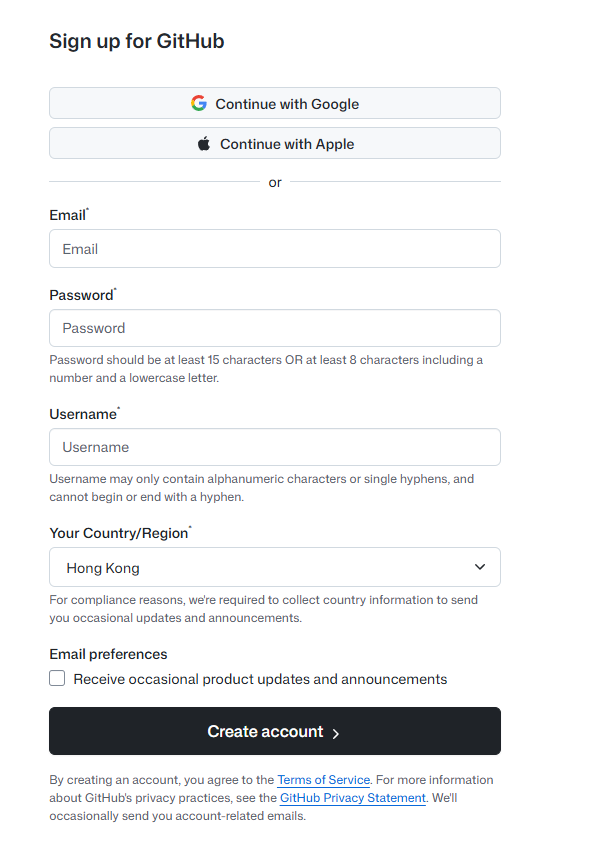
\includegraphics[width=0.5\textwidth]{installation/images/sign_up_page.png}
    \caption{GitHub Sign Up Page}
    \label{fig:github_signup}
\end{figure}

Then complete the registration form carefully by following these steps:

\begin{enumerate}
    \item In the \textbf{Email} field, use your official UMS email account.

    For example:
    \begin{quote}
        \texttt{ggg@iluv.ums.edu.my}
    \end{quote}
    where \texttt{ggg} should be replaced with your own UMS username.

    \item In the \textbf{Password} field, create a strong password.

    Your password should:
    \begin{itemize}
        \item contain a combination of uppercase and lowercase letters,
        \item include numbers and symbols,
        \item not be too short,
        \item not be something easy to guess such as your name or matric number.
    \end{itemize}

    \item In the \textbf{Username} field, choose a good and professional username.

    Please choose carefully because this account may be used in the future for public collaboration, portfolio work, open-source contribution, or job-related projects. A good username should:
    \begin{itemize}
        \item be simple,
        \item be professional,
        \item be easy to remember,
        \item avoid unnecessary symbols or random numbers unless needed.
    \end{itemize}

    Examples of suitable usernames:
    \begin{itemize}
        \item \texttt{ahmadrahman}
        \item \texttt{nuraisyah}
        \item \texttt{danielums}
        \item \texttt{farhan.dev}
    \end{itemize}

    \item Set the \textbf{Country} to \textbf{Malaysia}.

    \item Continue with the registration process by following all instructions shown in the browser.

    \item GitHub may ask you to complete one or more verification steps, for example:
    \begin{itemize}
        \item solving a simple puzzle,
        \item clicking a verification checkbox,
        \item confirming that you are not a robot,
        \item verifying your email address.
    \end{itemize}

    \item Read each instruction carefully and complete the verification until GitHub allows you to proceed.

    \item If you do not know what to do during any verification step, please ask my FYP student for assistance (YASMIN MADISIN REKY,RACHEL LINDA JANILON,MOHAMAD SUHAIMIE,FARRAH NABILA BINTI MAIDIN).

    \item Once all required information has been filled in and verification has been completed, finish the sign-up process until your account is created successfully.
\end{enumerate}

\subsection*{Verify that the account has been created successfully}

After registration, you must make sure that your GitHub account is really working.

\begin{enumerate}
    \item Log out first if GitHub logs you in automatically after sign-up.

    \item Go to the GitHub login page and sign in using the account that you have just created.

    \item Enter your registered email address and password.

    \item If login is successful, you should be able to enter your GitHub account homepage.

    \item You should also be able to see your profile icon or account menu on the top part of the page.

    \item This means that your GitHub account has been created successfully and is ready to use.

    \item If login fails, check the following:
    \begin{itemize}
        \item whether the email address is correct,
        \item whether the password is correct,
        \item whether email verification is still pending.
    \end{itemize}
\end{enumerate}

\section*{Course Repository}

Open the following repository link \href{https://github.com/project-with-student/computer_programming_25_26}{click\_me: Course Repository}. 

This repository is used as a companion resource for the \textbf{Basic Programming} tutorial sessions. It contains code examples, exercises, and supplementary materials to support students throughout the semester. The content will be updated from time to time.

\subsection*{What is a fork?}

For students who are using GitHub for the first time, it is important to understand what a \textbf{fork} is.

A \textbf{fork} is your own copy of someone else's repository under your personal GitHub account. When you fork a repository:

\begin{itemize}
    \item you get a copy of the original repository,
    \item the copy belongs to your GitHub account,
    \item you can work on it without changing the original repository directly,
    \item you can later sync your fork when the original repository is updated.
\end{itemize}

In this course, each student needs to fork the repository so that everyone has their own copy to work with.

\subsection*{How to fork the repository}
\begin{figure}
    \centering
    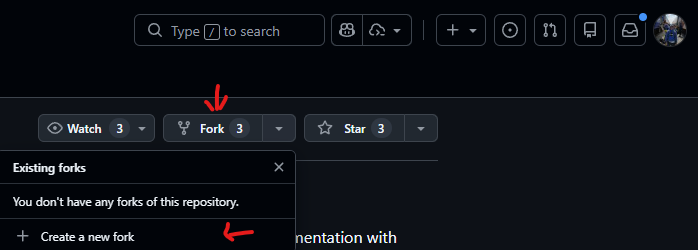
\includegraphics[width=0.5\textwidth]{installation/images/fork_button.png}
    \caption{Fork Button Location}
    \label{fig:fork_button}

\end{figure}

\begin{figure}
    \centering
    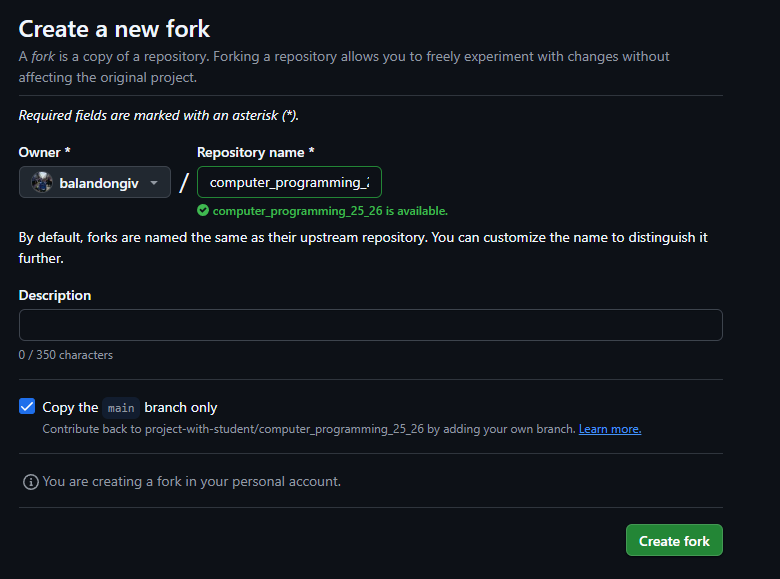
\includegraphics[width=0.5\textwidth]{installation/images/fork_setup.png}
    \caption{Create Fork Page}
    \label{fig:fork_setup}
\end{figure}
\begin{enumerate}

  
    \item Open the repository page \href{https://github.com/project-with-student/computer_programming_25_26}{click\_me: Course Repository}.
  
    \item Look at the top area of the repository page and find the \textbf{Fork} button as shown in  Figure~\ref{fig:fork_button}.

    \item Click the \textbf{Fork} button.Kindly refer to Figure~\ref{fig:fork_button} for the location of the Fork button.

    \item A small menu or page should appear. For first-time users, GitHub may show a message similar to:
    \begin{quote}
        \texttt{Existing forks} \\
        \texttt{You don't have any forks of this repository.} \\
        \texttt{Create a new fork}
    \end{quote}

    \item Click \textbf{Create a new fork}.

    \item GitHub will then open the fork creation page as shown in \ref{fig:fork_setup}.

    \item You may rename the repository to whatever you like. However, you may also keep the repository name as it is, which is usually the easiest option.

    \item After checking the repository name, click the \textbf{Create fork} button.

    \item Wait for GitHub to create the fork.

    \item A new page should appear after the forking process is completed.

    \item If you notice carefully, the page layout should look almost the same as the original repository page. This means that you now have an exact copy of the original repository under your own GitHub account as shown in Figure~\ref{fig:repo_ui}.

    \item You should also be able to see that the repository now belongs to your account, not only to the original owner.
\end{enumerate}

\begin{figure}
    \centering
    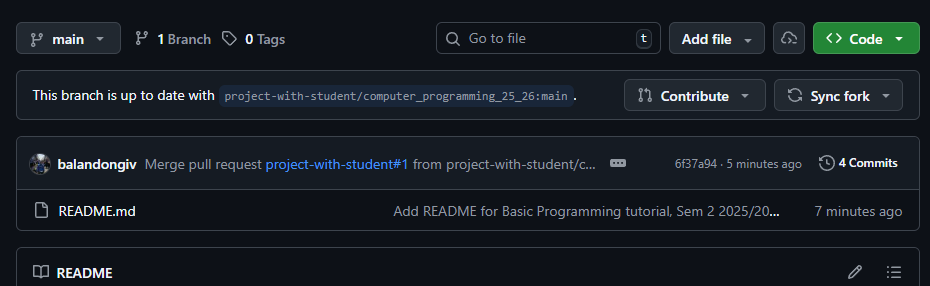
\includegraphics[width=0.5\textwidth]{installation/images/repo_ui.png}
    \caption{Forked Repository Page}
    \label{fig:repo_ui}
\end{figure}

\subsection*{Why the fork is important}

Forking is important in this course because:

\begin{itemize}
    \item you will have your own working copy of the repository,
    \item you can use Codespaces from your own copy,
    \item you can save your own progress safely,
    \item you can receive future updates from the original repository by syncing your fork.
\end{itemize}

\section*{Codespaces}

For this course, at the beginning, we will be using \href{https://github.com/features/codespaces}{GitHub Codespaces}.

GitHub Codespaces is a cloud-based development environment provided by GitHub. It allows students to write and run code directly in the browser without needing to perform full software installation on their own computers.

\subsection*{Why we use GitHub Codespaces}

The main advantage is that we do not need to do complicated setup at the beginning. Apart from that, GitHub Codespaces also provides other benefits:

\begin{itemize}
    \item \textbf{No local installation is needed.} Students do not need to install many tools manually before starting.
    \item \textbf{Same environment for everyone.} This reduces problems caused by different operating systems or software versions.
    \item \textbf{Accessible from anywhere.} Students can open their work from different computers as long as they can log in to GitHub.
    \item \textbf{Faster to start.} Students can focus on learning programming instead of spending too much time on configuration.
    \item \textbf{Better consistency.} The required packages and dependencies can already be prepared in advance.
    \item \textbf{Convenient for class use.} This makes it easier to follow tutorial sessions because everyone works in a similar environment.
\end{itemize}

\subsection*{How to open Codespaces}

After you have successfully forked the repository, open \textbf{your forked repository}, not the original repository.

Then follow these steps:
\begin{figure}
    \centering
    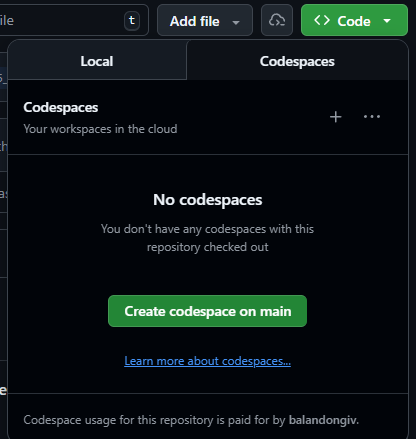
\includegraphics[width=0.5\textwidth]{installation/images/open_codespaces.png}
    \caption{Codespaces Tab Location}
    \label{fig:open_codespaces}
\end{figure}
\begin{enumerate}
    \item In your forked repository page, click the \textbf{Code} button. The button and UI is as shown in Figure~\ref{fig:open_codespaces}.

    \item A menu will appear with several tabs.

    \item Click the \textbf{Codespaces} tab.

    \item Then click \textbf{Create codespace on main}.

    \item After that, GitHub will start preparing the environment as shown in Figure~\ref{fig:loading_codespaces}.

    \item You will see a message or page indicating that Codespaces is opening.

    \item Wait until the Codespace finishes loading completely .

    \item Once it has opened, an automatic setup process may run for a while, about 10 minutes or more, depending on the server load and your internet connection.
    \item After the setup is complete, you should see the Codespaces interface as shown in Figure~\ref{fig:success_codespaces}.
\end{enumerate}
\begin{figure}
    \centering
    
\includegraphics[width=0.5\textwidth]{installation/images/loading_codespaces.png}
    \caption{Loading Codespaces}
    \label{fig:loading_codespaces}
\end{figure}

\begin{figure}
    \centering
    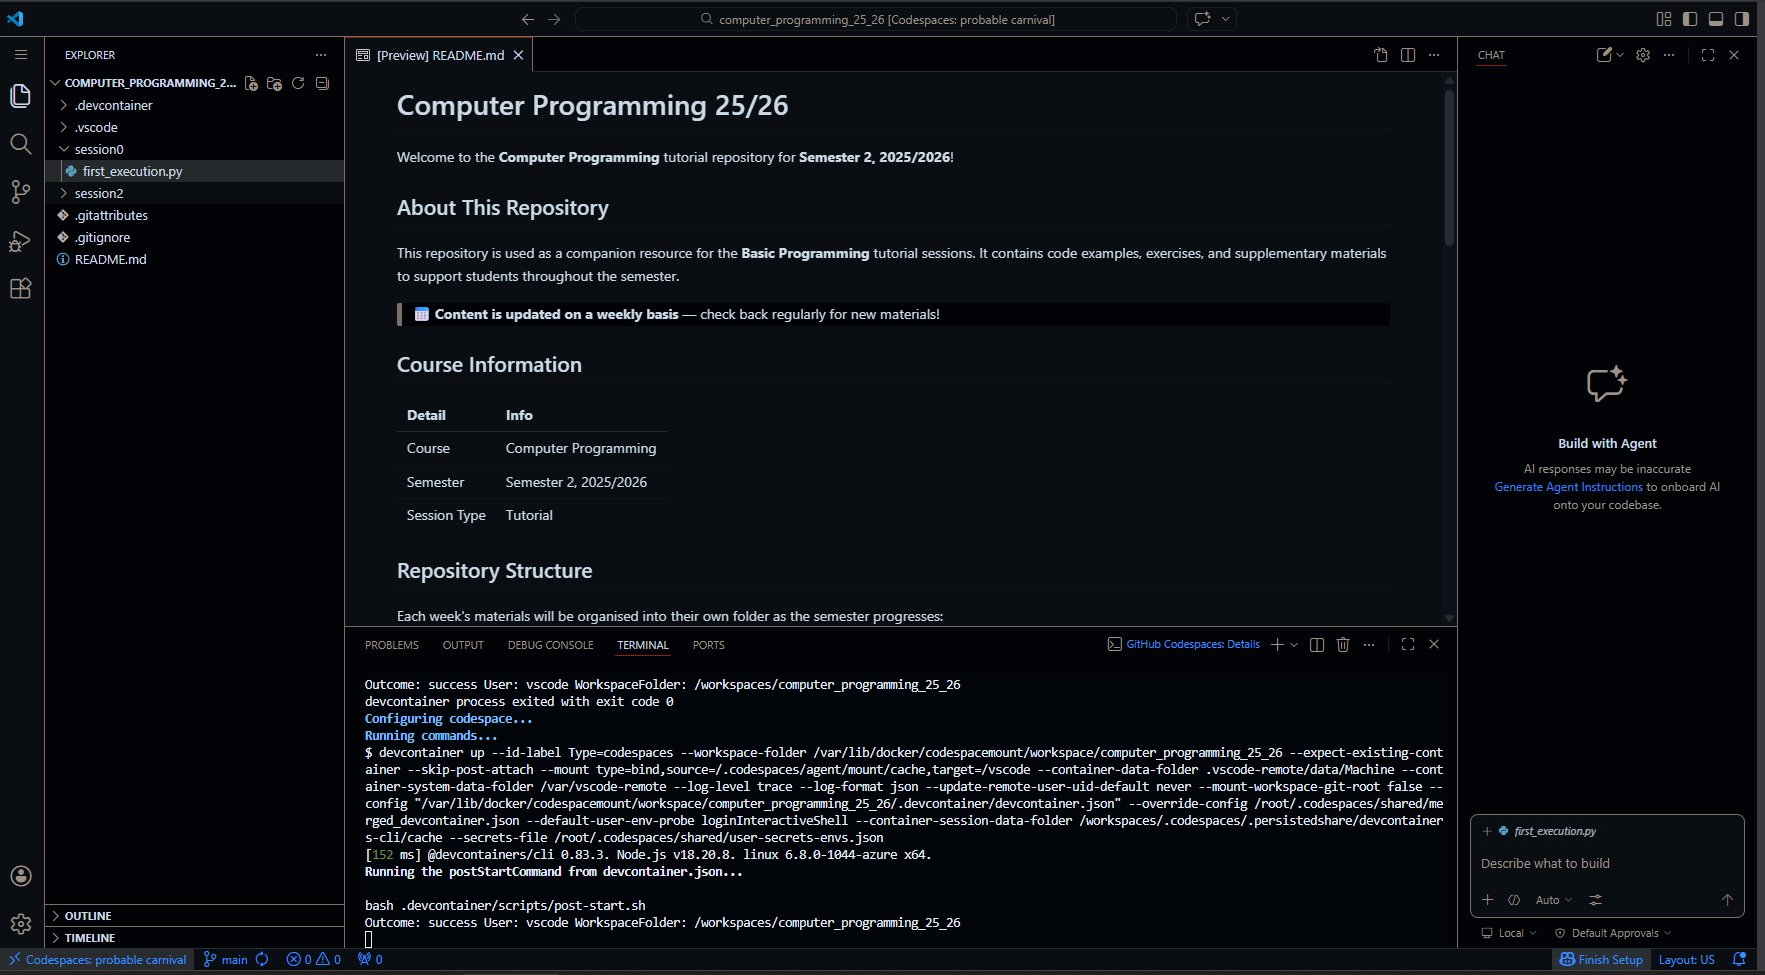
\includegraphics[width=0.5\textwidth]{installation/images/success_codespaces.png}
    \caption{Codespaces Successfully Opened}
    \label{fig:success_codespaces}
\end{figure}
\subsection*{Initial check inside Codespaces}

All the necessary packages should already have been installed for you.

To make sure everything is working correctly, first click the "Explorer" icon on the left sidebar to open the file explorer.
Then, locate the folder name "session0" and open it. Inside that folder, you should find a file named "first\_execution.py". Double click it.
\begin{figure}
    \centering
    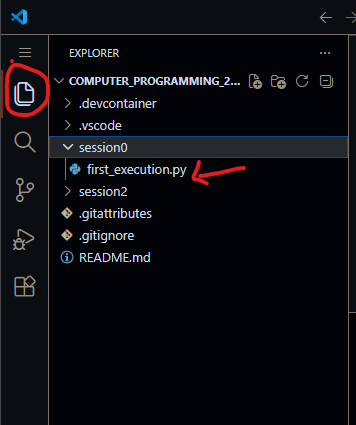
\includegraphics[width=0.5\textwidth]{installation/images/execute_final.png}
    \caption{Running the Initial Check Script}
    \label{fig:execute_final}
\end{figure}
Then, click the "Run" button at the top right corner of the editor as shown in Figure~\ref{fig:execute_final}.

The output should appear in the \ref{fig:execute_first_execution}
\begin{figure}
    \centering
    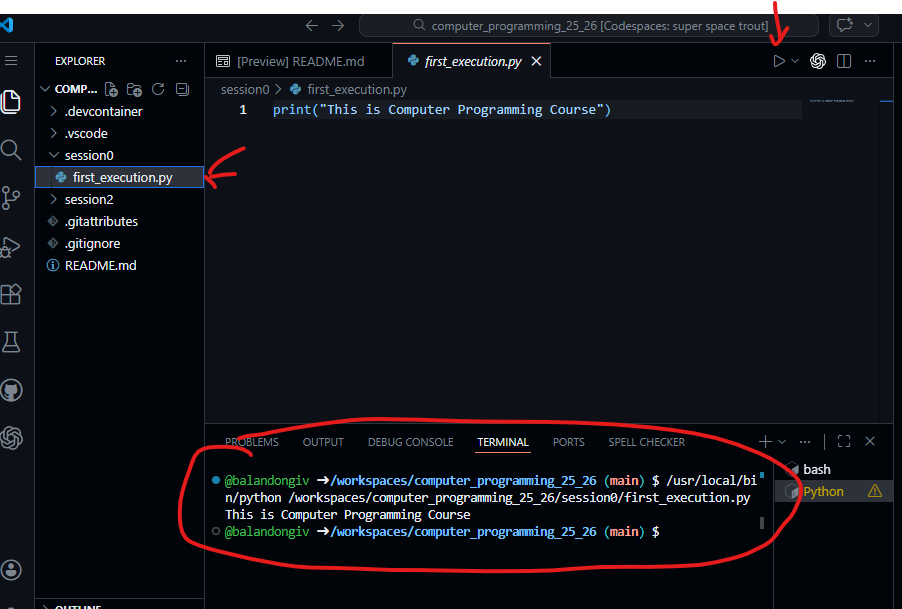
\includegraphics[width=0.5\textwidth]{installation/images/execute_first_execution.png}
    \caption{Running the Initial Check Script}
    \label{fig:execute_first_execution}

\end{figure}
\subsection*{If something does not work}

If the Codespace does not open properly, or if the script cannot be run:

\begin{itemize}
    \item check that you opened Codespaces from your own fork,
    \item refresh the page and wait again,
    \item make sure the terminal is active,
    \item try running the command again carefully,
    \item ask for help if you are not sure what went wrong.
\end{itemize}

\subsection*{Pulling new updates from the original repository}

As mentioned earlier, I will update the content of the repository from time to time. Therefore, you need to \textbf{sync} your fork so that your copy receives the latest updates.

\subsubsection{How to sync the fork on GitHub}

\begin{figure}
    \centering
    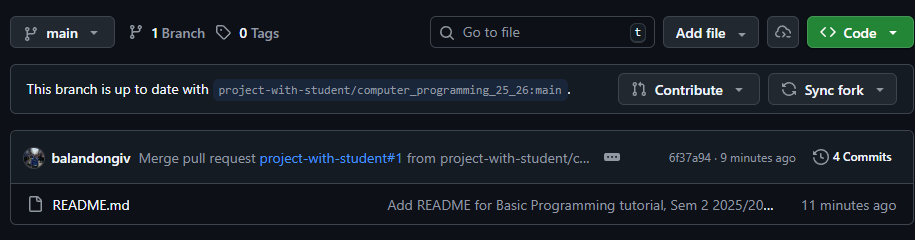
\includegraphics[width=0.5\textwidth]{installation/images/sync_fork.png}
    \caption{Sync Fork Button Location}
    \label{fig:sync_fork}
\end{figure}
\begin{enumerate}
    \item Open your forked repository on GitHub.

    \item Near the top area of the repository page, find the \textbf{Sync fork} button.

    \item Click \textbf{Sync fork}. The button and UI is as shown in Figure~\ref{fig:sync_fork}.

    \item If updates are available from the original repository, GitHub will give you the option to update your fork.

    \item Proceed with the sync action until your fork is updated.

    \item After the sync is successful, your fork will contain the latest content from the original repository.
\end{enumerate}

\subsubsection*{How to update your Codespace after syncing}

If your Codespace is already open when you sync the fork on GitHub, you should also update the files inside the Codespace.

\begin{enumerate}
    \item Return to your Codespace terminal.

    \item Run:
    \begin{quote}
        \texttt{git pull}
    \end{quote}

    \item Wait until the latest changes are downloaded into your Codespace.

    \item If needed, run \texttt{first\_run.py} again to make sure everything is still working correctly.
\end{enumerate}

\subsection*{Important reminder}

Throughout the semester, always remember the following workflow:

\begin{enumerate}
    \item Use your own GitHub account.
    \item Work from your own fork of the repository.
    \item Open Codespaces from your fork.
    \item Sync your fork whenever new course content is released.
    \item Pull the latest changes in Codespaces after syncing.
\end{enumerate}

\section*{How to Stop a GitHub Codespace to Save CPU/Compute Time}

To stop GitHub Codespaces from using compute or CPU time, you should \textbf{stop the codespace} when you are not using it. A stopped codespace keeps your saved work, but all running processes are halted, so compute usage stops.

\subsection*{Ways to Stop a Codespace}

\begin{itemize}
    \item \textbf{In the browser:} Open your codespace and choose \textbf{Stop codespace}.
    \item \textbf{In VS Code:} Open the Command Palette and select \texttt{Codespaces: Stop Codespace}.
    \item \textbf{Using the CLI:}
\end{itemize}

\begin{verbatim}
gh codespace stop
\end{verbatim}

Then choose the codespace you want to stop.

\subsection*{Important Details}

\begin{itemize}
    \item \textbf{Idle timeout:} Codespaces automatically stop after a period of inactivity. The default timeout is usually 30 minutes, and you can change this in your Codespaces settings for new codespaces.
    \item \textbf{Storage still remains:} Stopping a codespace saves compute time, but the codespace still uses storage until it is deleted. If you no longer need it, delete it to avoid storage charges.
\end{itemize}

\subsection*{Recommended Workflow}

\begin{enumerate}
    \item Commit and push your changes.
    \item Stop the codespace.
    \item Delete old unused codespaces to avoid storage costs.
\end{enumerate}